% IT Ethics: A Philosophical History of Information Technology
% Brendan Shea, PhD
% Rochester Community and Technical College

\documentclass[aspectratio=169]{beamer}

% Theme and colors
\usetheme{Madrid}
\usecolortheme{whale}
\setbeamertemplate{navigation symbols}{}
\setbeamertemplate{footline}[frame number]

% Packages
\usepackage[utf8]{inputenc}
\usepackage[T1]{fontenc}
\usepackage{graphicx}
\usepackage{booktabs}
\usepackage{array}
\usepackage{multirow}
\usepackage{hyperref}
\usepackage{csquotes}

% TikZ and libraries
\usepackage{tikz}
\usetikzlibrary{shapes.geometric, arrows.meta, positioning, calc, backgrounds, fit, decorations.pathreplacing, shadows, mindmap, trees}

% Custom colors
\definecolor{primaryblue}{RGB}{0,74,124}
\definecolor{accentorange}{RGB}{230,126,34}
\definecolor{lightgray}{RGB}{245,245,245}
\definecolor{darktext}{RGB}{44,62,80}


% Title information
\title[IT Ethics]{IT Ethics: A Philosophical History}
\subtitle{Technology, Power, and Human Choices}
\author{Brendan Shea, PhD}
\institute[RCTC]{Rochester Community and Technical College}
\date{}

\begin{document}

%------------------------------------------------------
% SLIDE 1: IT Ethics: Technology, Power, and Human Choices
%------------------------------------------------------
\begin{frame}
\titlepage
\end{frame}

\begin{frame}{IT Ethics: Technology, Power, and Human Choices}
    \begin{itemize}
        \item \textbf{Information Technology (IT)} refers to any tool or system humans use to create, store, communicate, or process information---from ancient writing to modern AI.
        \item Throughout history, new information technologies have transformed societies, economies, and the way humans relate to one another.
        \item Each technological revolution raises profound \textbf{ethical questions}: Who benefits? Who is harmed? Who controls access to information?
        \item This course examines five major IT revolutions to understand the challenges we face today with social media, AI, and digital platforms.
    \end{itemize}
    
    \vspace{0.5em}
    
    \begin{alertblock}{Core Question}
        How do we make wise choices about technologies that reshape what it means to be human?
    \end{alertblock}
\end{frame}

%------------------------------------------------------
% SLIDE 2: What Is Information Technology?
%------------------------------------------------------
\begin{frame}{What Is Information Technology?}
    \begin{itemize}
        \item \textbf{Information} is any data, knowledge, or content that can be communicated, stored, or processed by humans or machines.
        \item \textbf{Technology} comes from the Greek \textit{techne} (craft or skill) and refers to tools and techniques humans create to extend their capabilities.
        \item Information technology includes both \textbf{hardware} (physical tools like clay tablets, printing presses, and smartphones) and \textbf{software} (systems of symbols, codes, and procedures).
    \end{itemize}
    
    \vspace{0.3em}
    
    \begin{center}
    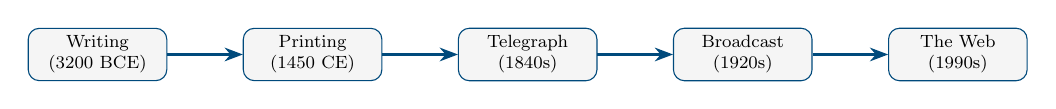
\begin{tikzpicture}[
        node distance=1.2cm,
        scale = .8,
        transform shape,
        every node/.style={font=\small},
        box/.style={rectangle, draw=primaryblue, fill=lightgray, rounded corners, minimum width=2.2cm, minimum height=0.8cm, align=center, font=\footnotesize}
    ]
        \node[box] (writing) {Writing\\(3200 BCE)};
        \node[box, right=of writing] (printing) {Printing\\(1450 CE)};
        \node[box, right=of printing] (telegraph) {Telegraph\\(1840s)};
        \node[box, right=of telegraph] (broadcast) {Broadcast\\(1920s)};
        \node[box, right=of broadcast] (web) {The Web\\(1990s)};
        
        \draw[-{Stealth}, thick, primaryblue] (writing) -- (printing);
        \draw[-{Stealth}, thick, primaryblue] (printing) -- (telegraph);
        \draw[-{Stealth}, thick, primaryblue] (telegraph) -- (broadcast);
        \draw[-{Stealth}, thick, primaryblue] (broadcast) -- (web);
    \end{tikzpicture}
    \end{center}
\end{frame}

%------------------------------------------------------
% SLIDE 3: What Is Ethics? (And Why Does IT Need It?)
%------------------------------------------------------
\begin{frame}{What Is Ethics? (And Why Does IT Need It?)}
    \begin{itemize}
        \item \textbf{Ethics} is the branch of philosophy that studies questions about right and wrong, good and bad, and how we ought to live and treat others.
        \item Unlike laws (which vary by country) or customs (which vary by culture), ethics asks what \textit{should} be the case, not just what \textit{is} the case.
        \item IT ethics matters because technology is never neutral---every design choice embeds values and affects who has power over information.
        \item We need ethical thinking because technology changes faster than laws, and engineers and users must make choices before regulators catch up.
    \end{itemize}
    
    \vspace{0.3em}
    
    \begin{exampleblock}{Example: The ``Like'' Button}
        Facebook's designers chose to create a ``Like'' button but no ``Dislike'' button. This design choice shapes how millions of people communicate, favoring positive reinforcement over critical feedback. Was this a neutral technical decision, or an ethical one?
    \end{exampleblock}
\end{frame}

%------------------------------------------------------
% SLIDE 4: Why Study History to Understand Today's Technology?
%------------------------------------------------------
\begin{frame}{Why Study History to Understand Today's Technology?}
    \begin{itemize}
        \item Every major information technology---from writing to social media---was once ``new,'' and each generated hopes, fears, and unintended consequences.
        \item Studying past IT revolutions reveals recurring patterns: promises of democratization, concerns about lost skills, debates over gatekeeping, and unforeseen harms.
        \item History helps us avoid both \textbf{techno-utopianism} (believing technology will automatically solve all problems) and \textbf{techno-pessimism} (believing technology is inherently destructive).
        \item By understanding how past societies navigated technological change, we gain perspective on our current choices about AI, social media, and digital privacy.
    \end{itemize}
    
    \vspace{0.3em}
    
    \begin{block}{George Santayana, \textit{The Life of Reason} (1905)}
        ``Those who cannot remember the past are condemned to repeat it.''
    \end{block}
\end{frame}

%------------------------------------------------------
% SLIDE 5: Five Revolutions in Information Technology
%------------------------------------------------------
\begin{frame}{Five Revolutions in Information Technology}
    \begin{itemize}
        \item A \textbf{technological revolution} occurs when a new tool fundamentally changes how societies create, store, and share information, reshaping power structures and daily life.
        \item Each revolution brings genuine benefits (wider access, new capabilities) alongside serious risks (new forms of control, unintended harms, lost skills).
        \item The five revolutions we will study span over 5,000 years, yet each raises surprisingly similar ethical questions about access, truth, and power.
        \item Understanding these patterns helps us recognize that today's debates about AI and social media are not entirely new---they echo ancient concerns.
    \end{itemize}
    
    \vspace{0.3em}
    
    \begin{table}[h]
        \centering
        \footnotesize
        \begin{tabular}{@{}lll@{}}
            \toprule
            \textbf{Revolution} & \textbf{Era} & \textbf{Key Innovation} \\
            \midrule
            Writing & 3200 BCE & External memory storage \\
            Printing Press & 1450 CE & Mass reproduction of texts \\
            Telegraph/Phone & 1840s--1870s & Instantaneous distance communication \\
            Broadcast Media & 1920s--1950s & One-to-many mass communication \\
            The World Wide Web & 1990s & Global networked information \\
            \bottomrule
        \end{tabular}
    \end{table}
\end{frame}

%------------------------------------------------------
% SLIDE 6: Recurring Questions: Gatekeepers, Memory, Unintended Consequences
%------------------------------------------------------
\begin{frame}{Recurring Questions: Gatekeepers, Memory, Unintended Consequences}
    \begin{itemize}
        \item \textbf{Gatekeeping}: Every IT system involves choices about who can create, access, and control information---from ancient scribes to modern platform algorithms.
        \item \textbf{Memory and Cognition}: Each new technology changes what humans need to remember and how we think, raising concerns about dependency and lost skills.
        \item \textbf{Unintended Consequences}: Technologies designed for one purpose often produce unexpected effects---the printing press enabled both the Scientific Revolution and devastating religious wars.
        \end{itemize}
    
    \vspace{0.3em}
    
    \begin{center}
    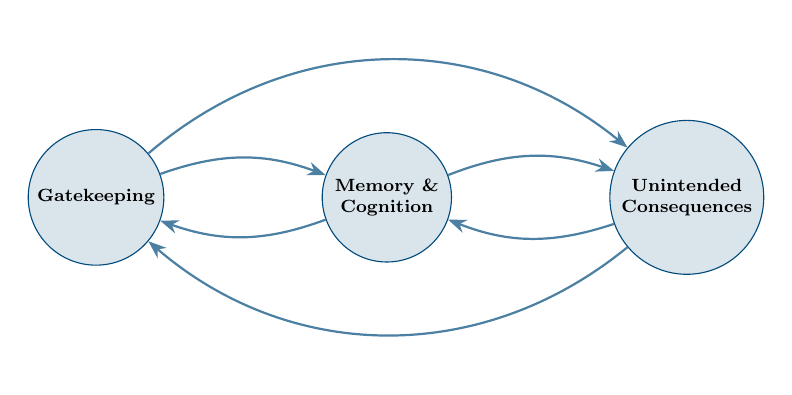
\begin{tikzpicture}[
        node distance=2.5cm,
        scale = .8,
        transform shape,
        concept/.style={circle, draw=primaryblue, fill=primaryblue!15, minimum size=2cm, align=center, font=\footnotesize\bfseries},
        arrow/.style={-{Stealth}, thick, primaryblue!70}
    ]
        \node[concept] (gate) {Gatekeeping};
        \node[concept, right=of gate] (memory) {Memory \&\\Cognition};
        \node[concept, right=of memory] (unintended) {Unintended\\Consequences};
        
        \draw[arrow, bend left=20] (gate) to (memory);
        \draw[arrow, bend left=20] (memory) to (gate);
        \draw[arrow, bend left=20] (memory) to (unintended);
        \draw[arrow, bend left=20] (unintended) to (memory);
        \draw[arrow, bend left=40] (gate) to (unintended);
        \draw[arrow, bend left=40] (unintended) to (gate);
    \end{tikzpicture}
    \end{center}
\end{frame}

%------------------------------------------------------
% SLIDE 7: The First Revolution: Writing
%------------------------------------------------------
\begin{frame}{The First Revolution: Writing}
    \begin{itemize}
        \item \textbf{Writing} is a system of visual symbols that represents spoken language, allowing information to be stored outside the human mind for the first time.
        \item Writing emerged independently in at least three locations: Mesopotamia (cuneiform, c.\ 3200 BCE), Egypt (hieroglyphics, c.\ 3200 BCE), and China (oracle bones, c.\ 1200 BCE).
        \item This technology solved a fundamental problem: human memory is limited, fallible, and dies with the individual, but written records can persist for millennia.
        \item The invention of writing marks the boundary between \textbf{prehistory} (known only through archaeology) and \textbf{history} (known through written records).
    \end{itemize}
    
    \vspace{0.3em}
    
    \begin{alertblock}{A Radical Change}
        For the first time, knowledge could travel across space without a messenger and across time without continuous oral transmission. This single innovation made civilization as we know it possible.
    \end{alertblock}
\end{frame}

%------------------------------------------------------
% SLIDE 8: Before Writing: How Oral Cultures Preserved Knowledge
%------------------------------------------------------
\begin{frame}{Before Writing: How Oral Cultures Preserved Knowledge}
    \begin{itemize}
        \item \textbf{Oral cultures} relied entirely on human memory and face-to-face communication to preserve and transmit knowledge across generations.
        \item These societies developed sophisticated techniques for memory: rhythm, rhyme, repetition, formulaic phrases, and narrative structures that made information memorable.
        \item Epic poems like the \textit{Iliad} and \textit{Odyssey} were composed and transmitted orally for centuries before being written down, using metrical patterns as memory aids.
        \item Oral transmission required active participation---listeners became tellers---creating a dynamic, living tradition rather than a fixed text.
    \end{itemize}
    
    \vspace{0.3em}
    
    \begin{block}{Characteristics of Oral vs.\ Literate Cultures}
        \begin{itemize}
            \item \textbf{Oral}: Knowledge is embodied in people; learning requires personal relationships; traditions evolve organically with each retelling.
            \item \textbf{Literate}: Knowledge exists in objects; learning can occur alone; texts remain fixed but may lose living context.
        \end{itemize}
    \end{block}
\end{frame}

%------------------------------------------------------
% SLIDE 9: The Invention of Writing: Mesopotamia, Egypt, China
%------------------------------------------------------
\begin{frame}{The Invention of Writing: Mesopotamia, Egypt, China}
    \begin{itemize}
        \item \textbf{Cuneiform} (Mesopotamia, c.\ 3200 BCE) began as pictographs on clay tablets for recording trade and taxes, evolving into wedge-shaped marks representing sounds.
        \item \textbf{Hieroglyphics} (Egypt, c.\ 3200 BCE) combined pictorial symbols with phonetic elements, used for religious texts, monuments, and administration.
        \item \textbf{Chinese script} (c.\ 1200 BCE) developed from oracle bone inscriptions used for divination, becoming a logographic system still in use today.
        \item In each case, writing emerged first to serve practical needs---accounting, religion, governance---before expanding to literature, history, and philosophy.
    \end{itemize}
    
    \vspace{0.3em}
    
    \begin{table}[h]
        \centering
        \footnotesize
        \begin{tabular}{@{}llll@{}}
            \toprule
            \textbf{System} & \textbf{Region} & \textbf{Date} & \textbf{Original Purpose} \\
            \midrule
            Cuneiform & Mesopotamia & c.\ 3200 BCE & Trade records, taxes \\
            Hieroglyphics & Egypt & c.\ 3200 BCE & Religious texts, monuments \\
            Oracle Bone & China & c.\ 1200 BCE & Divination, royal records \\
            \bottomrule
        \end{tabular}
    \end{table}
\end{frame}

%------------------------------------------------------
% SLIDE 10: Plato's Phaedrus: An Ancient Philosopher Worries About Technology
%------------------------------------------------------
\begin{frame}{Plato's \textit{Phaedrus}: An Ancient Philosopher Worries About Technology}
    \begin{itemize}
        \item \textbf{Plato} (c.\ 428--348 BCE) was an Athenian philosopher and student of Socrates who founded the Academy, one of the first institutions of higher learning in the Western world.
        \item The \textit{Phaedrus} (c.\ 370 BCE) is a dialogue in which Socrates discusses love, rhetoric, and---crucially for us---the dangers of the new technology of writing.
        \item Socrates tells the myth of \textbf{Theuth and Thamus}: Theuth, an Egyptian god, invents writing and presents it to King Thamus as a gift that will improve memory and wisdom.
        \item King Thamus disagrees, arguing that writing will have the opposite effect---weakening memory and creating only the \textit{appearance} of wisdom.
    \end{itemize}
    
    \vspace{0.3em}
    
    \begin{exampleblock}{Historical Context}
        In Socrates's Athens (5th century BCE), writing was still relatively new for philosophical discourse. Most teaching happened through oral dialogue, and many Greeks viewed written texts with suspicion.
    \end{exampleblock}
\end{frame}

%------------------------------------------------------
% SLIDE 11: Socrates's Argument: Writing Will Destroy Memory
%------------------------------------------------------
\begin{frame}{Socrates's Argument: Writing Will Destroy Memory}
    \begin{itemize}
        \item Socrates argues that writing creates \textbf{external dependence}: people will trust written symbols ``which are no part of themselves'' instead of cultivating their own internal memory.
        \item Writing produces the \textbf{appearance of wisdom} without the reality---readers will ``appear to be omniscient'' while actually knowing nothing deeply.
        \item Unlike a living teacher, a written text cannot respond to questions, clarify misunderstandings, or adapt its message to the needs of different learners.
        \item Socrates compares writing to painting: both seem alive, but ``if you ask them a question they preserve a solemn silence.''
    \end{itemize}
    
    \vspace{0.3em}
    
    \begin{block}{Plato, \textit{Phaedrus} (c.\ 370 BCE)}
        ``This discovery of yours will create forgetfulness in the learners' souls, because they will not use their memories; they will trust to the external written characters and not remember of themselves.''
    \end{block}
\end{frame}

%------------------------------------------------------
% SLIDE 12: The Irony: We Only Know This Because Plato Wrote It Down
%------------------------------------------------------
\begin{frame}{The Irony: We Only Know This Because Plato Wrote It Down}
    \begin{itemize}
        \item Socrates himself never wrote anything---all of his ideas survive only because his student Plato chose to write them down in dialogue form.
        \item This creates a profound \textbf{performative contradiction}: the argument against writing is preserved and transmitted across 2,400 years \textit{because it was written}.
        \item If Plato had followed Socrates's advice and refused to write, we would know nothing of Socrates's philosophy, including his critique of writing itself.
        \item This irony suggests that the relationship between technology and human flourishing is more complex than simple acceptance or rejection.
    \end{itemize}
    
    \vspace{0.3em}
    
    \begin{center}
    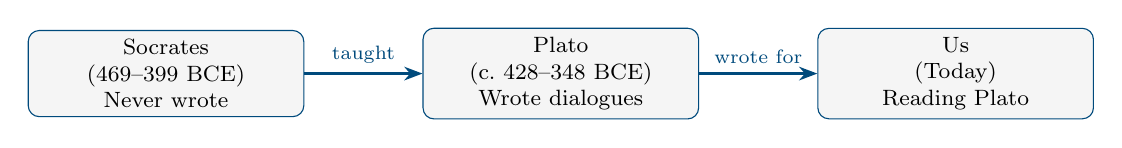
\begin{tikzpicture}[
        node distance=0.8cm,
        box/.style={rectangle, draw=primaryblue, fill=lightgray, rounded corners, minimum width=3.5cm, minimum height=1cm, align=center, font=\footnotesize}
    ]
        \node[box] (socrates) {Socrates\\(469--399 BCE)\\Never wrote};
        \node[box, right=1.5cm of socrates] (plato) {Plato\\(c.\ 428--348 BCE)\\Wrote dialogues};
        \node[box, right=1.5cm of plato] (us) {Us\\(Today)\\Reading Plato};
        
        \draw[-{Stealth}, thick, primaryblue] (socrates) -- node[above, font=\scriptsize] {taught} (plato);
        \draw[-{Stealth}, thick, primaryblue] (plato) -- node[above, font=\scriptsize] {wrote for} (us);
    \end{tikzpicture}
    \end{center}
\end{frame}

%------------------------------------------------------
% SLIDE 13: Writing and Empire: Bureaucracy, Law Codes, and Power
%------------------------------------------------------
\begin{frame}{Writing and Empire: Bureaucracy, Law Codes, and Power}
    \begin{itemize}
        \item Writing enabled \textbf{bureaucracy}---the administration of complex societies through standardized records of taxes, land ownership, military service, and legal judgments.
        \item The earliest law codes, such as the \textbf{Code of Hammurabi} (c.\ 1754 BCE), used writing to make laws public, permanent, and (theoretically) applicable to all citizens equally.
        \item Empires from Assyria to Rome depended on written communication to coordinate armies, collect tribute, and govern distant provinces without the ruler being physically present.
        \item Writing created a new class of \textbf{gatekeepers}---scribes and priests who controlled access to literacy and thus wielded enormous social power.
    \end{itemize}
    
    \vspace{0.3em}
    
    \begin{alertblock}{The Double Edge of Written Law}
        Written law codes made rules transparent and consistent---but they also enabled more systematic control over populations. The same technology that protects citizens' rights can enforce totalitarian rule.
    \end{alertblock}
\end{frame}

%------------------------------------------------------
% SLIDE 14: Discussion: What Does the Writing Revolution Teach Us?
%------------------------------------------------------
\begin{frame}{Discussion: What Does the Writing Revolution Teach Us?}
    \begin{itemize}
        \item Socrates worried that writing would make people dependent on external memory and give them false confidence in their own knowledge.
        \item Writing enabled unprecedented preservation of knowledge, coordination of complex societies, and the rule of law---but also new forms of surveillance and control.
        \item The ``scribal class'' became powerful gatekeepers, controlling who could access and produce written information.
        \item Every benefit of writing (permanence, reach, precision) came with a corresponding risk (rigidity, loss of context, exclusion of the illiterate).
    \end{itemize}
    
    \vspace{0.3em}
    
    \begin{block}{Discussion Questions}
        \begin{enumerate}
            \item Was Socrates right that we lose something important when we externalize memory? Think about GPS, calculators, and search engines.
            \item Who are today's ``scribes''---the gatekeepers who control access to information technology?
            \item Can you think of a modern technology that, like writing, has both liberated and controlled people?
        \end{enumerate}
    \end{block}
\end{frame}

%------------------------------------------------------
% SLIDE 15: The Second Revolution: The Printing Press
%------------------------------------------------------
\begin{frame}{The Second Revolution: The Printing Press}
    \begin{itemize}
        \item For over 4,000 years after writing was invented, every copy of a text had to be made by hand---a slow, expensive, error-prone process that kept books rare and costly.
        \item \textbf{Johannes Gutenberg} (c.\ 1400--1468) developed \textbf{movable type} printing in Mainz, Germany around 1450, enabling the mass production of identical texts.
        \item The printing press reduced the cost of books by roughly 80\% within its first century, transforming who could access written knowledge.
        \item This revolution in information technology would reshape religion, science, politics, and culture in ways Gutenberg never imagined or intended.
    \end{itemize}
    
    \vspace{0.3em}
    
    \begin{center}
    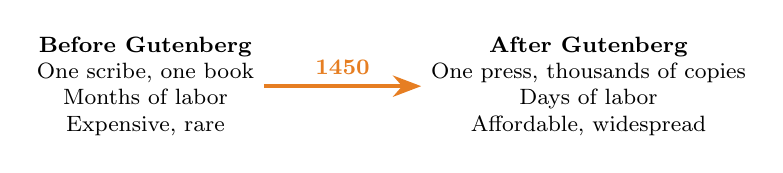
\begin{tikzpicture}[
        node distance=0.6cm,
        every node/.style={font=\footnotesize}
    ]
        \node[align=center] (before) {\textbf{Before Gutenberg}\\One scribe, one book\\Months of labor\\Expensive, rare};
        \node[right=2cm of before, align=center] (after) {\textbf{After Gutenberg}\\One press, thousands of copies\\Days of labor\\Affordable, widespread};
        
        \draw[-{Stealth}, ultra thick, accentorange] (before) -- node[above, font=\footnotesize\bfseries] {1450} (after);
    \end{tikzpicture}
    \end{center}
\end{frame}

%------------------------------------------------------
% SLIDE 16: Gutenberg's Innovation: Movable Type (1450s)
%------------------------------------------------------
\begin{frame}{Gutenberg's Innovation: Movable Type (1450s)}
    \begin{itemize}
        \item \textbf{Movable type} uses individual letter blocks that can be arranged, inked, pressed onto paper, and then rearranged to print different texts.
        \item Gutenberg combined several existing technologies: the screw press (from wine-making), oil-based ink, and metal alloy letter molds that could produce thousands of identical characters.
        \item The \textbf{Gutenberg Bible} (c.\ 1455) was the first major book printed with movable type in Europe, demonstrating that printed books could match the quality of hand-copied manuscripts.
        \item Within 50 years, printing presses spread across Europe; by 1500, an estimated 20 million volumes had been printed---more than all the manuscripts produced in the previous thousand years.
    \end{itemize}
    
    \vspace{0.3em}
    
    \begin{exampleblock}{A System, Not Just a Machine}
        Gutenberg's genius was not inventing any single component, but integrating existing technologies into a \textit{system} for mass production. This pattern---combining existing tools in new ways---recurs throughout the history of IT innovation.
    \end{exampleblock}
\end{frame}

%------------------------------------------------------
% SLIDE 17: What Changed: Books Become Cheap and Abundant
%------------------------------------------------------
\begin{frame}{What Changed: Books Become Cheap and Abundant}
    \begin{itemize}
        \item Before printing, a single book might cost as much as a house---each copy required months of labor by trained scribes working in monastery scriptoriums.
        \item The printing press reduced the cost of books by approximately 80\% within its first century, making written knowledge accessible to merchants, professionals, and eventually ordinary citizens.
        \item By 1500---just 50 years after Gutenberg---an estimated 20 million books had been printed in Europe, more than all manuscripts produced in the previous thousand years combined.
        \item This flood of books created new industries (publishing, bookselling), new professions (editors, typesetters), and new problems (piracy, misinformation, censorship).
    \end{itemize}
    
    \vspace{0.3em}
    
    \begin{table}[h]
        \centering
        \footnotesize
        \begin{tabular}{@{}lll@{}}
            \toprule
            \textbf{Year} & \textbf{Print Centers} & \textbf{Estimated Books Printed} \\
            \midrule
            1455 & 1 (Mainz) & First Bible printed \\
            1480 & 110+ cities & Millions of pages \\
            1500 & 250+ cities & $\sim$20 million volumes \\
            \bottomrule
        \end{tabular}
    \end{table}
\end{frame}

%------------------------------------------------------
% SLIDE 18: Erasmus: The Dream of the "Republic of Letters"
%------------------------------------------------------
\begin{frame}{Erasmus: The Dream of the ``Republic of Letters''}
    \begin{itemize}
        \item \textbf{Desiderius Erasmus} (c.\ 1466--1536) was a Dutch humanist scholar who became the first intellectual celebrity of the print age, with over 3,000 surviving letters connecting scholars across Europe.
        \item Erasmus championed the \textbf{Republic of Letters} (\textit{Respublica Litteraria})---an ideal community of scholars who would share knowledge across national and religious boundaries through reasoned dialogue.
        \item He believed the printing press could spread education, reform the Church gradually through scholarship, and create a cosmopolitan culture of learning transcending political divisions.
        \item Erasmus used the press strategically: publishing accessible textbooks, a Greek New Testament, and carefully crafted letters that shaped his public image as a voice of moderation.
    \end{itemize}
    
    \vspace{0.3em}
    
    \begin{block}{The Humanist Vision}
        Erasmus imagined print as a tool for \textit{gradual} reform through education and persuasion. He believed that if people could read the Bible and classical texts for themselves, reason would prevail over superstition and corruption.
    \end{block}
\end{frame}

%------------------------------------------------------
% SLIDE 19: Martin Luther: The First Viral Media Campaign
%------------------------------------------------------
\begin{frame}{Martin Luther: The First Viral Media Campaign}
    \begin{itemize}
        \item \textbf{Martin Luther} (1483--1546) was a German monk and professor whose \textbf{95 Theses} (1517), criticizing the sale of indulgences, spread across Europe within weeks thanks to the printing press.
        \item Unlike previous reformers who were easily silenced, Luther's ideas could not be suppressed once thousands of printed copies circulated---he became, in effect, the first ``viral'' author.
        \item Luther invented the \textbf{pamphlet} (\textit{Flugschriften}, or ``flying writings''): short, cheap, vernacular documents that could be produced in days and read aloud in ten minutes.
        \item By 1521, Luther had published more works than any author since the invention of printing; between 1517 and 1520, his pamphlets ran through 370 editions totaling nearly 400,000 copies.
    \end{itemize}
    
    \vspace{0.3em}
    
    \begin{exampleblock}{A New Kind of Writing}
        Luther's \textit{Sermon on Indulgences and Grace} (1518) was only 1,500 words---divided into 20 short paragraphs anyone could understand. It was reprinted 14 times in its first year alone.
    \end{exampleblock}
\end{frame}

%------------------------------------------------------
% SLIDE 20: The Good: Vernacular Bibles, Scientific Revolution, Mass Literacy
%------------------------------------------------------
\begin{frame}{The Good: Vernacular Bibles, Scientific Revolution, Mass Literacy}
    \begin{itemize}
        \item The printing press enabled \textbf{vernacular Bibles}---translations into German, English, French, and other languages---allowing ordinary people to read scripture without relying on clergy as intermediaries.
        \item The \textbf{Scientific Revolution} depended on print: Copernicus, Galileo, and Newton could share precise diagrams, tables, and mathematical proofs that were reproduced identically across thousands of copies.
        \item Print created demand for \textbf{mass literacy}: as books became affordable, reading became a practical skill for merchants, craftsmen, and eventually children in newly established schools.
        \item Standardization of texts meant that scholars in London and Prague could discuss the exact same edition, enabling collaborative knowledge-building across vast distances.
    \end{itemize}
    
    \vspace{0.3em}
    
    \begin{center}
    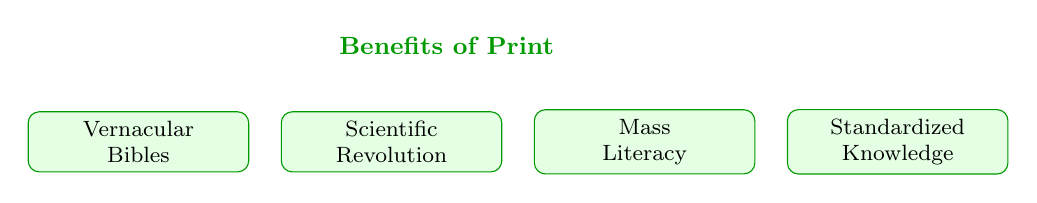
\begin{tikzpicture}[
        node distance=0.5cm,
        box/.style={rectangle, draw=green!60!black, fill=green!10, rounded corners, minimum width=2.8cm, minimum height=0.7cm, align=center, font=\footnotesize}
    ]
        \node[box] (bible) {Vernacular\\Bibles};
        \node[box, right=0.4cm of bible] (science) {Scientific\\Revolution};
        \node[box, right=0.4cm of science] (literacy) {Mass\\Literacy};
        \node[box, right=0.4cm of literacy] (standard) {Standardized\\Knowledge};
        
        \node[above=0.6cm of science, xshift=0.7cm, font=\small\bfseries, text=green!60!black] {Benefits of Print};
    \end{tikzpicture}
    \end{center}
\end{frame}

%------------------------------------------------------
% SLIDE 21: The Dark Side: Propaganda, Conspiracy, and Witch-Hunting Manuals
%------------------------------------------------------
\begin{frame}{The Dark Side: Propaganda, Conspiracy, and Witch-Hunting Manuals}
    \begin{itemize}
        \item The same technology that spread scientific knowledge and vernacular Bibles also mass-produced \textbf{propaganda}, conspiracy theories, and instructions for persecution.
        \item The \textit{Malleus Maleficarum} (``Hammer of Witches,'' 1487) became one of the most reprinted books in Europe, providing detailed instructions for identifying and prosecuting ``witches.''
        \item Pamphlets spread false accusations against religious minorities, including blood libel myths claiming Jews murdered Christian children---lies that fueled pogroms across Europe.
        \item Print made rumors permanent and portable: a lie could now travel faster than any correction, reaching audiences who would never encounter a rebuttal.
    \end{itemize}
    
    \vspace{0.3em}
    
    \begin{alertblock}{A Sobering Lesson}
        The printing press did not distinguish between true and false, helpful and harmful. It amplified \textit{whatever people wanted to read}---including hatred, fear, and superstition.
    \end{alertblock}
\end{frame}

%------------------------------------------------------
% SLIDE 22: Luther's On the Jews and Their Lies: When Ideas Have Consequences
%------------------------------------------------------
\begin{frame}{Luther's \textit{On the Jews and Their Lies}: When Ideas Have Consequences}
    \begin{itemize}
        \item In 1543, Martin Luther published \textit{On the Jews and Their Lies}, a 65,000-word treatise calling for the destruction of synagogues, confiscation of Jewish property, and forced labor or expulsion.
        \item Luther recommended that synagogues and schools ``be set on fire,'' homes ``razed and destroyed,'' and rabbis ``forbidden to teach henceforth on pain of loss of life and limb.''
        \item The printing press ensured this text survived and spread for centuries; four hundred years later, the Nazis displayed it at Nuremberg rallies and cited it to justify anti-Jewish legislation.
        \item This case illustrates a crucial point: the same person can produce both liberating ideas (religious reform) and deeply harmful ones---and print preserves both equally.
    \end{itemize}
    
    \vspace{0.3em}
    
    \begin{block}{Historical Consequence}
        Kristallnacht (November 9--10, 1938)---when Nazis burned synagogues across Germany---occurred on Luther's birthday. Bishop Martin Sasse published a pamphlet connecting Luther's 1543 recommendations to their ``fulfillment'' by the Nazis.
    \end{block}
\end{frame}

%------------------------------------------------------
% SLIDE 23: The Thirty Years' War: Information Technology and Mass Death
%------------------------------------------------------
\begin{frame}{The Thirty Years' War: Information Technology and Mass Death}
    \begin{itemize}
        \item The \textbf{Thirty Years' War} (1618--1648) was one of the most destructive conflicts in European history, killing an estimated 4.5 to 8 million people---approximately 20\% of the German population.
        \item The war began as a religious conflict between Catholics and Protestants, fueled by decades of printed propaganda, pamphlet wars, and competing interpretations of scripture.
        \item Printed materials dehumanized enemies, spread atrocity stories (real and fabricated), and made compromise seem like betrayal of sacred principles.
        \item The Peace of Westphalia (1648) ended the war but settled religious questions almost exactly as they had been resolved in 1555---before the bloodshed began.
    \end{itemize}
    
    \vspace{0.3em}
    
    \begin{center}
    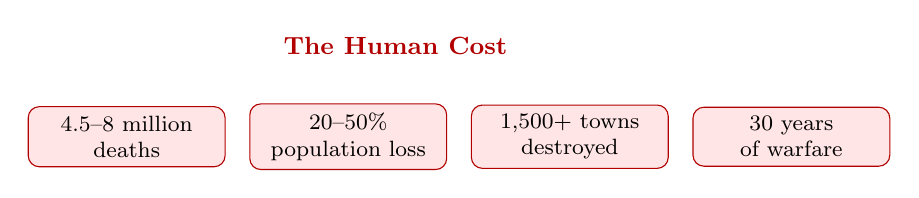
\begin{tikzpicture}[
        node distance=0.4cm,
        box/.style={rectangle, draw=red!70!black, fill=red!10, rounded corners, minimum width=2.5cm, minimum height=0.6cm, align=center, font=\footnotesize}
    ]
        \node[box] (deaths) {4.5--8 million\\deaths};
        \node[box, right=0.3cm of deaths] (pop) {20--50\%\\population loss};
        \node[box, right=0.3cm of pop] (cities) {1,500+ towns\\destroyed};
        \node[box, right=0.3cm of cities] (years) {30 years\\of warfare};
        
        \node[above=0.5cm of pop, xshift=0.6cm, font=\small\bfseries, text=red!70!black] {The Human Cost};
    \end{tikzpicture}
    \end{center}
\end{frame}

%------------------------------------------------------
% SLIDE 24: Discussion: What Does the Printing Press Teach Us?
%------------------------------------------------------
\begin{frame}{Discussion: What Does the Printing Press Teach Us?}
    \begin{itemize}
        \item The printing press enabled the Scientific Revolution, mass literacy, and religious reform---but also propaganda, conspiracy theories, and religious wars that killed millions.
        \item Erasmus dreamed of a ``Republic of Letters'' where scholars would share knowledge peacefully; Luther showed that print could bypass gatekeepers and reach mass audiences directly.
        \item The technology itself was neutral; its effects depended on what people chose to print, who could afford to publish, and what audiences wanted to read.
        \item The gap between Gutenberg (1450) and the Peace of Westphalia (1648) was almost 200 years---societies needed generations to develop new norms, institutions, and literacies.
    \end{itemize}
    
    \vspace{0.3em}
    
    \begin{block}{Discussion Questions}
        \begin{enumerate}
            \item What parallels do you see between the printing press and social media? What's different?
            \item Luther's ideas spread because they resonated with what people already felt. Is ``going viral'' more about the message or the medium?
            \item If it took 200 years to adapt to print, how long might it take to adapt to digital media?
        \end{enumerate}
    \end{block}
\end{frame}

%------------------------------------------------------
% SLIDE 25: The Third Revolution: Telegraph, Telephone, and Mass Literacy
%------------------------------------------------------
\begin{frame}{The Third Revolution: Telegraph, Telephone, and Mass Literacy}
    \begin{itemize}
        \item The \textbf{long nineteenth century} (roughly 1789--1914) saw an explosion of new information technologies that shrank distances and expanded access to knowledge.
        \item The \textbf{telegraph} (1840s) enabled near-instantaneous communication across continents---the first time information could travel faster than a human being.
        \item The \textbf{telephone} (1876) made real-time voice communication possible, transforming business, government, and personal relationships.
        \item \textbf{Mass literacy campaigns} and compulsory education created millions of new readers, while cheap newspapers (the ``penny press'') made daily news accessible to working people.
    \end{itemize}
    
    \vspace{0.3em}
    
    \begin{center}
    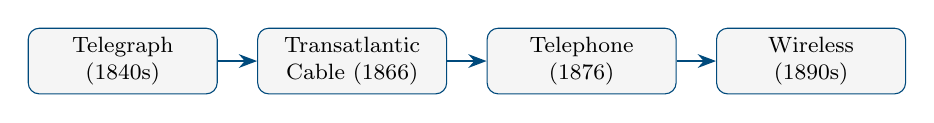
\begin{tikzpicture}[
        node distance=0.8cm,
        box/.style={rectangle, draw=primaryblue, fill=lightgray, rounded corners, minimum width=2.4cm, minimum height=0.7cm, align=center, font=\footnotesize}
    ]
        \node[box] (telegraph) {Telegraph\\(1840s)};
        \node[box, right=0.5cm of telegraph] (cable) {Transatlantic\\Cable (1866)};
        \node[box, right=0.5cm of cable] (phone) {Telephone\\(1876)};
        \node[box, right=0.5cm of phone] (radio) {Wireless\\(1890s)};
        
        \draw[-{Stealth}, thick, primaryblue] (telegraph) -- (cable);
        \draw[-{Stealth}, thick, primaryblue] (cable) -- (phone);
        \draw[-{Stealth}, thick, primaryblue] (phone) -- (radio);
    \end{tikzpicture}
    \end{center}
\end{frame}

%------------------------------------------------------
% SLIDE 26: New Technologies: Shrinking the World
%------------------------------------------------------
\begin{frame}{New Technologies: Shrinking the World}
    \begin{itemize}
        \item Before the telegraph, news from London to New York took at least ten days by ship; after the transatlantic cable (1866), it took minutes.
        \item These technologies created new industries (news agencies, telephone companies), new professions (telegraph operators, telephone switchboard workers), and new forms of crime (wire fraud).
        \item Governments quickly recognized the strategic importance of communication infrastructure---controlling telegraph lines became as important as controlling roads and ports.
        \item The dream of ``annihilating distance'' inspired utopian hopes that faster communication would promote peace, understanding, and global unity.
    \end{itemize}
    
    \vspace{0.3em}
    
    \begin{exampleblock}{The First ``World Wide Web''}
        By 1900, undersea telegraph cables connected every continent except Antarctica. Victorian commentators called this network the ``nervous system of the world''---a metaphor strikingly similar to how we describe the internet today.
    \end{exampleblock}
\end{frame}

%------------------------------------------------------
% SLIDE 27: The Rise of Mass Education and Cheap Newspapers
%------------------------------------------------------
\begin{frame}{The Rise of Mass Education and Cheap Newspapers}
    \begin{itemize}
        \item Throughout the 19th century, European and American governments introduced \textbf{compulsory education}, creating the first mass literate populations in human history.
        \item Literacy rates in Western Europe rose from roughly 50\% in 1800 to over 90\% by 1900, transforming who could participate in public discourse.
        \item The \textbf{penny press} (newspapers sold for one cent) emerged in the 1830s, replacing expensive papers aimed at elites with cheap dailies covering crime, scandal, and human interest stories.
        \item Mass literacy created a new kind of public: millions of readers who could be informed, persuaded, entertained---or manipulated---through print.
    \end{itemize}
    
    \vspace{0.3em}
    
    \begin{table}[h]
        \centering
        \footnotesize
        \begin{tabular}{@{}lll@{}}
            \toprule
            \textbf{Country} & \textbf{Literacy c.\ 1800} & \textbf{Literacy c.\ 1900} \\
            \midrule
            England & $\sim$55\% & $\sim$97\% \\
            France & $\sim$40\% & $\sim$95\% \\
            Germany & $\sim$60\% & $\sim$99\% \\
            United States & $\sim$75\% & $\sim$90\% \\
            \bottomrule
        \end{tabular}
    \end{table}
\end{frame}

%------------------------------------------------------
% SLIDE 28: John Stuart Mill: The Marketplace of Ideas
%------------------------------------------------------
\begin{frame}{John Stuart Mill: The Marketplace of Ideas}
    \begin{itemize}
        \item \textbf{John Stuart Mill} (1806--1873) was an English philosopher whose essay \textit{On Liberty} (1859) became the most influential defense of free speech in the Western tradition.
        \item Mill argued that society should allow the free expression of all opinions, even false or offensive ones, because open debate is the best method for discovering truth.
        \item His key insight: if an opinion is true, silencing it robs humanity of truth; if it is false, refuting it strengthens our understanding of why the truth is true.
        \item Mill believed that ``the collision of adverse opinions'' would gradually lead society toward progress, enlightenment, and human flourishing.
    \end{itemize}
    
    \vspace{0.3em}
    
    \begin{block}{John Stuart Mill, \textit{On Liberty} (1859)}
        ``If all mankind minus one, were of one opinion, and only one person were of the contrary opinion, mankind would be no more justified in silencing that one person, than he, if he had the power, would be justified in silencing mankind.''
    \end{block}
\end{frame}

%------------------------------------------------------
% SLIDE 29: Mill's Liberal Optimism: More Speech, More Truth, More Progress
%------------------------------------------------------
\begin{frame}{Mill's Liberal Optimism: More Speech, More Truth, More Progress}
    \begin{itemize}
        \item Mill's vision was profoundly optimistic: he believed that over time, free debate would lead humanity toward greater truth, tolerance, and moral progress.
        \item He argued that even false opinions serve a purpose---they force defenders of truth to sharpen their arguments and avoid ``dead dogma'' (beliefs held without understanding).
        \item Mill trusted that ordinary people, given access to information and education, would generally make good decisions about what to believe and how to live.
        \item This \textbf{liberal optimism} shaped democratic theory: the best response to bad speech is more speech, not censorship.
    \end{itemize}
    
    \vspace{0.3em}
    
    \begin{block}{Mill's Three-Part Defense of Free Speech}
        \begin{itemize}
            \item If the silenced opinion is \textbf{true}, we lose the chance to exchange error for truth.
            \item If the silenced opinion is \textbf{false}, we lose the chance to strengthen our understanding of the truth through debate.
            \item If the silenced opinion is \textbf{partly true}, we lose the portion of truth it contains.
        \end{itemize}
    \end{block}
\end{frame}

%------------------------------------------------------
% SLIDE 30: Karl Marx: Who Owns the Means of Communication?
%------------------------------------------------------
\begin{frame}{Karl Marx: Who Owns the Means of Communication?}
    \begin{itemize}
        \item \textbf{Karl Marx} (1818--1883) was a German philosopher and economist who developed a powerful critique of capitalism and its effects on politics, culture, and ideas.
        \item Marx agreed with Mill that free expression was essential, calling it ``the realization of human freedom'' and arguing that ``the absence of freedom of the press makes all other freedoms illusory.''
        \item However, Marx asked a question Mill largely ignored: \textit{Who owns the printing presses, newspapers, and telegraph lines?} Who can afford to publish?
        \item Marx argued that formal freedom of speech means little if the \textbf{means of communication} are controlled by wealthy elites who shape what ideas reach the public.
    \end{itemize}
    
    \vspace{0.3em}
    
    \begin{alertblock}{The Structural Question}
        Mill asked: ``Should we allow people to speak?'' Marx asked: ``Who actually \textit{can} speak---and who gets heard?''
    \end{alertblock}
\end{frame}

%------------------------------------------------------
% SLIDE 31: Marx's Challenge: "Free Press" Means Freedom for Those Who Own Presses
%------------------------------------------------------
\begin{frame}{Marx's Challenge: ``Free Press'' Means Freedom for Those Who Own Presses}
    \begin{itemize}
        \item Marx argued that in a capitalist society, the class that controls \textbf{material production} (factories, land, capital) also controls \textbf{mental production} (newspapers, books, ideas).
        \item The ``marketplace of ideas'' is not a level playing field: some voices are amplified by wealth and institutional power, while others are marginalized or silenced by poverty.
        \item Marx did not oppose free speech---he was a crusading journalist who clashed repeatedly with government censors---but he insisted that ownership shapes content.
        \item This critique remains relevant: today, a handful of corporations control most newspapers, television networks, and social media platforms.
    \end{itemize}
    
    \vspace{0.3em}
    
    \begin{block}{Karl Marx \& Friedrich Engels, \textit{The German Ideology} (1846)}
        ``The ideas of the ruling class are in every epoch the ruling ideas... The class which has the means of material production at its disposal, has control at the same time over the means of mental production.''
    \end{block}
\end{frame}

%------------------------------------------------------
% SLIDE 32: World War I: When Communication Technology Becomes a Weapon
%------------------------------------------------------
\begin{frame}{World War I: When Communication Technology Becomes a Weapon}
    \begin{itemize}
        \item World War I (1914--1918) was the first major conflict coordinated by telegraph and telephone, allowing generals to command armies across continents in real time.
        \item Governments created the first modern \textbf{propaganda agencies}: the Committee on Public Information (US), the War Propaganda Bureau (UK), and equivalents in Germany and France.
        \item Cryptography became militarily critical---the interception and decoding of the \textbf{Zimmermann Telegram} (1917) helped bring the United States into the war.
        \item The war that was supposed to be ``over by Christmas'' killed approximately 20 million people, demonstrating that faster communication does not guarantee wiser decisions.
    \end{itemize}
    
    \vspace{0.3em}
    
    \begin{center}
    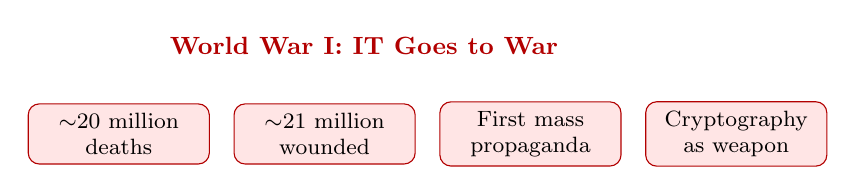
\begin{tikzpicture}[
        node distance=0.4cm,
        box/.style={rectangle, draw=red!70!black, fill=red!10, rounded corners, minimum width=2.3cm, minimum height=0.6cm, align=center, font=\footnotesize}
    ]
        \node[box] (dead) {$\sim$20 million\\deaths};
        \node[box, right=0.3cm of dead] (wounded) {$\sim$21 million\\wounded};
        \node[box, right=0.3cm of wounded] (prop) {First mass\\propaganda};
        \node[box, right=0.3cm of prop] (crypto) {Cryptography\\as weapon};
        
        \node[above=0.5cm of wounded, xshift=0.5cm, font=\small\bfseries, text=red!70!black] {World War I: IT Goes to War};
    \end{tikzpicture}
    \end{center}
\end{frame}

%------------------------------------------------------
% SLIDE 33: Propaganda, Cryptography, and Twenty Million Dead
%------------------------------------------------------
\begin{frame}{Propaganda, Cryptography, and Twenty Million Dead}
    \begin{itemize}
        \item World War I demonstrated that information technology could be weaponized on an industrial scale---not just for military coordination, but for shaping public opinion.
        \item Governments employed professional propagandists, poster artists, filmmakers, and journalists to demonize enemies, glorify sacrifice, and suppress dissent.
        \item \textbf{Cryptography} became a strategic asset: the British decryption of the Zimmermann Telegram (revealing German plans to ally with Mexico against the US) helped bring America into the war.
        \item The ``war to end all wars'' showed that Mill's optimism about the marketplace of ideas had limits: populations could be manipulated into supporting catastrophic decisions.
    \end{itemize}
    
    \vspace{0.3em}
    
    \begin{exampleblock}{The Zimmermann Telegram (1917)}
        British codebreakers intercepted and decrypted a German telegram proposing a military alliance with Mexico. When published in American newspapers, it shifted US public opinion toward entering the war---demonstrating that control over information could change history.
    \end{exampleblock}
\end{frame}

%------------------------------------------------------
% SLIDE 34: Discussion: What Does the Nineteenth Century Teach Us?
%------------------------------------------------------
\begin{frame}{Discussion: What Does the Nineteenth Century Teach Us?}
    \begin{itemize}
        \item Mill believed free and open debate would lead toward truth and progress; Marx warned that those who own the means of communication shape what ideas get heard.
        \item New technologies (telegraph, telephone, mass newspapers) promised to connect humanity and spread enlightenment---but also enabled unprecedented propaganda and mass warfare.
        \item The ``marketplace of ideas'' metaphor assumes a level playing field; in reality, access to communication has always been shaped by wealth, power, and institutional control.
        \item World War I revealed that faster communication does not guarantee wiser decisions---and that information can be weaponized against democratic deliberation.
    \end{itemize}
    
    \vspace{0.3em}
    
    \begin{block}{Discussion Questions}
        \begin{enumerate}
            \item Is the internet more like Mill's marketplace of ideas or Marx's analysis of media ownership? Can it be both?
            \item What modern examples show information technology being used for propaganda? How can citizens protect themselves?
            \item If faster communication doesn't guarantee better decisions, what else is needed for democratic deliberation to work?
        \end{enumerate}
    \end{block}
\end{frame}

%------------------------------------------------------
% SLIDE 35: The Fourth Revolution: Radio, Film, and Television
%------------------------------------------------------
\begin{frame}{The Fourth Revolution: Radio, Film, and Television}
    \begin{itemize}
        \item The 20th century introduced \textbf{broadcast media}: technologies that allowed a single source to reach millions of people simultaneously with sound and moving images.
        \item \textbf{Radio} (1920s) brought news, entertainment, and political speeches directly into homes; \textbf{film} created a new form of mass storytelling and propaganda.
        \item \textbf{Television} (1950s) combined the immediacy of radio with the visual power of film, becoming the dominant medium for news, politics, and culture by the 1960s.
        \item These technologies created \textbf{one-to-many communication} on an unprecedented scale: a handful of broadcasters could shape what entire nations saw, heard, and believed.
    \end{itemize}
    
    \vspace{0.3em}
    
    \begin{center}
    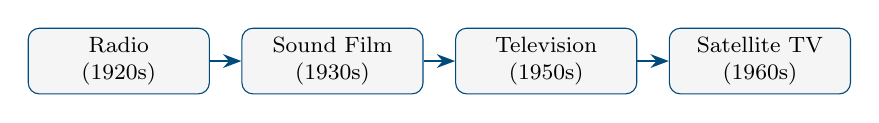
\begin{tikzpicture}[
        node distance=0.6cm,
        box/.style={rectangle, draw=primaryblue, fill=lightgray, rounded corners, minimum width=2.3cm, minimum height=0.7cm, align=center, font=\footnotesize}
    ]
        \node[box] (radio) {Radio\\(1920s)};
        \node[box, right=0.4cm of radio] (film) {Sound Film\\(1930s)};
        \node[box, right=0.4cm of film] (tv) {Television\\(1950s)};
        \node[box, right=0.4cm of tv] (satellite) {Satellite TV\\(1960s)};
        
        \draw[-{Stealth}, thick, primaryblue] (radio) -- (film);
        \draw[-{Stealth}, thick, primaryblue] (film) -- (tv);
        \draw[-{Stealth}, thick, primaryblue] (tv) -- (satellite);
    \end{tikzpicture}
    \end{center}
\end{frame}


%------------------------------------------------------
% NEW SLIDES FOR INSERTION BETWEEN SLIDES 35 AND 36
% These cover WWII-era mass media and the birth of computers
%------------------------------------------------------

%------------------------------------------------------
% NEW SLIDE A: WWII Mass Media: The Battle for Hearts and Minds
%------------------------------------------------------
\begin{frame}{WWII Mass Media: The Battle for Hearts and Minds}
    \begin{itemize}
        \item World War II (1939--1945) was the first war fought as much through radio waves as through bullets---both sides recognized that controlling information meant controlling morale.
        \item \textbf{Nazi Germany}: Propaganda Minister Joseph Goebbels declared radio ``the eighth great power'' and claimed the Nazi revolution ``would have been impossible without the radio.''
        \item \textbf{United States}: President Franklin D. Roosevelt used his ``Fireside Chats'' (1933--1944) to speak directly to citizens, bypassing newspapers and calming fears during the Depression and war.
        \item \textbf{Britain}: The BBC broadcast resistance messages to occupied Europe; listening to foreign broadcasts was punishable by death in Nazi Germany.
    \end{itemize}
    
    \vspace{0.3em}
    
    \begin{alertblock}{The Same Technology, Different Purposes}
        Radio could unite a nation against tyranny (FDR, BBC) or indoctrinate a population into supporting genocide (Goebbels). The technology itself was neutral---its effects depended on who controlled it and for what purposes.
    \end{alertblock}
\end{frame}

%------------------------------------------------------
% NEW SLIDE B: Radio for Democracy and Dictatorship
%------------------------------------------------------
\begin{frame}{Radio for Democracy and Dictatorship}
    \begin{itemize}
        \item \textbf{The Volksempf\"anger} (``People's Receiver''): Goebbels commissioned cheap radios (76 Reichsmarks, payable in installments) so every German home could receive Nazi broadcasts.
        \item By 1939, over 70\% of German households owned radios---deliberately limited in range to prevent listening to foreign stations like the BBC.
        \item \textbf{FDR's Fireside Chats}: Roosevelt's 31 radio addresses reached up to 60 million listeners, using conversational language to explain complex policies and restore confidence.
        \item Both leaders understood that radio's intimacy---a voice speaking directly into your living room---created an emotional bond impossible through print.
    \end{itemize}
    
    \vspace{0.3em}
    
    \begin{table}[h]
        \centering
        \footnotesize
        \begin{tabular}{p{3.2cm}p{3.2cm}p{3.2cm}}
            \toprule
            & \textbf{Nazi Germany} & \textbf{United States} \\
            \midrule
            Goal & Indoctrination & Informed citizenship \\
            Style & Rallies, spectacle & Conversational, intimate \\
            Foreign broadcasts & Banned (death penalty) & Allowed \\
            Outcome & Complicity in atrocity & Democratic mobilization \\
            \bottomrule
        \end{tabular}
    \end{table}
\end{frame}

%------------------------------------------------------
% NEW SLIDE C: The Birth of the Computer: Codebreaking and War
%------------------------------------------------------
\begin{frame}{The Birth of the Computer: Codebreaking and War}
    \begin{itemize}
        \item The first electronic digital computers were born not from peacetime research but from the urgent need to break enemy codes during World War II.
        \item \textbf{Bletchley Park}: A secret British facility where mathematicians, linguists, and engineers---75\% of them women---worked to crack Nazi communications.
        \item \textbf{Colossus} (1944): The world's first programmable digital electronic computer, designed by engineer Tommy Flowers to break the German Lorenz cipher used by Hitler's high command.
        \item \textbf{ENIAC} (1946): The American Electronic Numerical Integrator and Computer, originally designed to calculate artillery firing tables, became operational after the war ended.
    \end{itemize}
    
    \vspace{0.3em}
    
    \begin{center}
    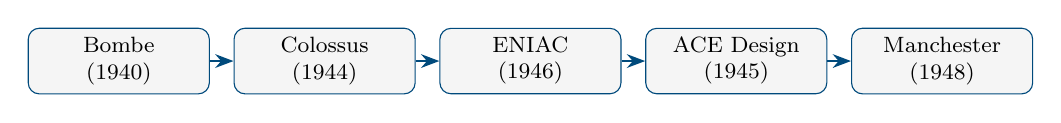
\begin{tikzpicture}[
        node distance=0.5cm,
        box/.style={rectangle, draw=primaryblue, fill=lightgray, rounded corners, minimum width=2.3cm, minimum height=0.6cm, align=center, font=\footnotesize}
    ]
        \node[box] (bombe) {Bombe\\(1940)};
        \node[box, right=0.3cm of bombe] (colossus) {Colossus\\(1944)};
        \node[box, right=0.3cm of colossus] (eniac) {ENIAC\\(1946)};
        \node[box, right=0.3cm of eniac] (ace) {ACE Design\\(1945)};
        \node[box, right=0.3cm of ace] (manchester) {Manchester\\(1948)};
        
        \draw[-{Stealth}, thick, primaryblue] (bombe) -- (colossus);
        \draw[-{Stealth}, thick, primaryblue] (colossus) -- (eniac);
        \draw[-{Stealth}, thick, primaryblue] (eniac) -- (ace);
        \draw[-{Stealth}, thick, primaryblue] (ace) -- (manchester);
    \end{tikzpicture}
    \end{center}
\end{frame}

%------------------------------------------------------
% NEW SLIDE D: Alan Turing and the Foundations of Computing
%------------------------------------------------------
\begin{frame}{Alan Turing and the Foundations of Computing}
    \begin{itemize}
        \item \textbf{Alan Turing} (1912--1954) was a British mathematician whose 1936 paper ``On Computable Numbers'' described a theoretical ``universal machine'' that could compute anything computable---the conceptual foundation of all modern computers.
        \item At Bletchley Park, Turing designed the \textbf{Bombe}, an electromechanical machine that cracked the German Enigma cipher, and contributed key insights to breaking the Lorenz cipher.
        \item After the war, Turing designed the \textbf{Automatic Computing Engine (ACE)}, one of the first designs for a stored-program computer---inspired by his wartime experience with Colossus.
        \item Tragically, Turing was prosecuted for homosexuality in 1952, chemically castrated, and died in 1954. The British government apologized in 2009; he was posthumously pardoned in 2013.
    \end{itemize}
 
    
    \begin{exampleblock}{From Codebreaking to Computing}
        \small
        The connection between wartime codebreaking and peacetime computing was direct: many pioneers of digital computers---Turing, Newman, Flowers---came from Bletchley Park. Information technology was born, in part, from the need to process enemy secrets faster than humans could.
    \end{exampleblock}
\end{frame}

%------------------------------------------------------
% SLIDE 36: Claude Shannon: A Mathematical Definition of Information
%------------------------------------------------------
\begin{frame}{Claude Shannon: A Mathematical Definition of Information}
    \begin{itemize}
        \item \textbf{Claude Shannon} (1916--2001) was an American mathematician and engineer whose 1948 paper ``A Mathematical Theory of Communication'' founded the field of \textbf{information theory}.
        \item Shannon defined \textbf{information} mathematically as the reduction of uncertainty---the more surprising a message, the more information it carries.
        \item He introduced the \textbf{bit} (binary digit) as the fundamental unit of information and showed how to calculate the minimum bits needed to transmit any message.
        \item Crucially, Shannon's definition separates information from \textit{meaning}: his theory measures how much data is transmitted, not whether it is true, important, or valuable.
    \end{itemize}
    
    \vspace{0.3em}
    
    \begin{alertblock}{The Semantic Gap}
        Shannon explicitly bracketed questions of meaning: ``The semantic aspects of communication are irrelevant to the engineering problem.'' His theory enables the internet, but cannot tell us whether what we communicate is wise, true, or good.
    \end{alertblock}
\end{frame}

%------------------------------------------------------
% SLIDE 37: Hannah Arendt: Mass Media and Totalitarianism
%------------------------------------------------------
\begin{frame}{Hannah Arendt: Mass Media and Totalitarianism}
    \begin{itemize}
        \item \textbf{Hannah Arendt} (1906--1975) was a German-American political philosopher who fled Nazi Germany and later wrote \textit{The Origins of Totalitarianism} (1951).
        \item Arendt analyzed how radio, film, and print propaganda enabled the rise of Nazism and Stalinism by creating \textbf{mass societies} of isolated individuals hungry for belonging.
        \item She observed that totalitarian propaganda works not by making people believe lies, but by creating \textbf{cynicism}---a world where people believe ``everything and nothing.''
        \item The ``ideal subject'' of totalitarian rule is someone for whom the distinction between \textbf{fact and fiction} no longer exists---making them easy to manipulate.
    \end{itemize}
    
    \vspace{0.3em}
    
    \begin{block}{Arendt on ``Mass Society''}
        Arendt argued that modern technology and urbanization created ``mass societies'' of atomized individuals---lonely, disconnected from community, and desperate for meaning. Totalitarian movements offered belonging, purpose, and a coherent story about the world---even if that story was built on lies.
    \end{block}
\end{frame}

%------------------------------------------------------
% SLIDE 38: Arendt's Warning: When Facts No Longer Matter
%------------------------------------------------------
\begin{frame}{Arendt's Warning: When Facts No Longer Matter}
    \begin{itemize}
        \item Arendt observed that constant lying by propaganda does not make people believe the lies---instead, it destroys their capacity to distinguish truth from falsehood.
        \item When proven wrong, followers don't abandon leaders; they ``take refuge in cynicism'' and admire their leaders' ``superior tactical cleverness.''
        \item The goal of totalitarian propaganda is not persuasion but \textbf{organization}---creating a movement where loyalty to the leader replaces independent thought.
        \item Arendt's analysis helps explain why simply ``fact-checking'' propaganda often fails to change minds.
    \end{itemize}
    
    \vspace{0.3em}
    
    \begin{alertblock}{Arendt on the ``Ideal Subject''}
        ``The ideal subject of totalitarian rule is not the convinced Nazi or the convinced Communist, but people for whom the distinction between fact and fiction (i.e., the reality of experience) and the distinction between true and false (i.e., the standards of thought) no longer exist.''
        
        \hfill---Hannah Arendt, \textit{The Origins of Totalitarianism} (1951)
    \end{alertblock}
\end{frame}

%------------------------------------------------------
% SLIDE 39: Neil Postman: Amusing Ourselves to Death
%------------------------------------------------------
\begin{frame}{Neil Postman: Amusing Ourselves to Death}
    \begin{itemize}
        \item \textbf{Neil Postman} (1931--2003) was an American media theorist whose 1985 book \textit{Amusing Ourselves to Death} critiqued the effects of television on public discourse.
        \item Postman contrasted two dystopian visions: George Orwell's \textit{1984} (control through pain and censorship) vs.\ Aldous Huxley's \textit{Brave New World} (control through pleasure and distraction).
        \item He argued that television transforms all content---news, politics, religion, education---into \textbf{entertainment}, making serious discourse impossible.
        \item Postman's central thesis: we are not being oppressed by tyrants, but are voluntarily ``amusing ourselves to death'' through passive consumption of trivial content.
    \end{itemize}
    
    \vspace{0.3em}
    
    \begin{exampleblock}{Two Dystopias}
        \textbf{Orwell's Fear}: An external tyrant bans books, controls information, and rules through fear.\\[0.3em]
        \textbf{Huxley's Fear}: No tyrant is needed---people willingly surrender autonomy because they are too distracted and entertained to care about truth.
    \end{exampleblock}
\end{frame}

%------------------------------------------------------
% SLIDE 40: Postman's Challenge: What If Huxley Was Right?
%------------------------------------------------------
\begin{frame}{Postman's Challenge: What If Huxley Was Right?}
    \begin{itemize}
        \item Postman argued that by 1985, Huxley's vision was proving more accurate than Orwell's: no government needed to censor us because we had stopped wanting to read.
        \item Television created a culture where ``the truth would be drowned in a sea of irrelevance''---not hidden, but buried under endless entertainment.
        \item The medium itself shapes the message: TV favors images over arguments, emotion over logic, and entertainment over substance---regardless of content.
        \item Postman's analysis anticipated concerns about social media: infinite distraction, shortened attention spans, and the transformation of citizenship into spectatorship.
    \end{itemize}
    
    \vspace{0.3em}
    
    \begin{quotation}
        ``What Orwell feared were those who would ban books. What Huxley feared was that there would be no reason to ban a book, for there would be no one who wanted to read one. \ldots\ Orwell feared that what we fear will ruin us. Huxley feared that what we desire will ruin us.''
        
        \hfill---Neil Postman, \textit{Amusing Ourselves to Death} (1985)
    \end{quotation}
\end{frame}

%------------------------------------------------------
% SLIDE 41: Discussion: What Does the Analog Era Teach Us?
%------------------------------------------------------
\begin{frame}{Discussion: What Does the Analog Era Teach Us?}
    \begin{itemize}
        \item Shannon showed us how to measure and transmit information with mathematical precision---but his theory deliberately ignores questions of meaning, truth, and value.
        \item Arendt warned that broadcast media could enable totalitarianism by creating cynical, atomized masses who believe ``everything and nothing.''
        \item Postman argued that television transforms all content into entertainment, making us passive consumers rather than active citizens.
        \item Both Arendt and Postman suggest that the \textit{medium itself}---not just the content---shapes how we think and relate to each other.
    \end{itemize}
    
    \vspace{0.3em}
    
    \begin{block}{Discussion Questions}
        \begin{enumerate}
            \item Are social media platforms more like Orwell's dystopia (surveillance, censorship) or Huxley's (distraction, entertainment)? Could they be both?
            \item Does the ``semantic gap'' in Shannon's theory matter? Can we build ethical communication systems without addressing meaning?
            \item How would Arendt analyze the spread of misinformation on social media? What would she say about ``post-truth'' politics?
        \end{enumerate}
    \end{block}
\end{frame}

%------------------------------------------------------
% SLIDE 42: The Fifth Revolution: Web 1.0
%------------------------------------------------------
\begin{frame}{The Fifth Revolution: Web 1.0}
    \begin{itemize}
        \item In 1989, British scientist \textbf{Tim Berners-Lee} proposed the \textbf{World Wide Web} while working at CERN, the European particle physics laboratory in Switzerland.
        \item Unlike previous revolutions where new technology was owned by elites (presses, broadcast licenses), the web was designed to be \textbf{open and decentralized}.
        \item By 1993, CERN released the web's underlying code as \textbf{royalty-free open source}, allowing anyone to create websites and browsers without permission or payment.
        \item \textbf{Web 1.0} (roughly 1990--2005) was characterized by static websites, limited interactivity, and the separation of ``content creators'' from ``consumers.''
    \end{itemize}
    
    \vspace{0.3em}
    
    \begin{center}
    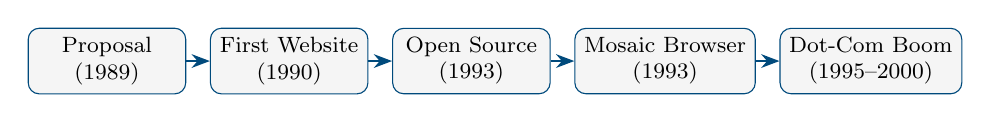
\begin{tikzpicture}[
        node distance=0.5cm,
        box/.style={rectangle, draw=primaryblue, fill=lightgray, rounded corners, minimum width=2cm, minimum height=0.6cm, align=center, font=\footnotesize}
    ]
        \node[box] (proposal) {Proposal\\(1989)};
        \node[box, right=0.3cm of proposal] (first) {First Website\\(1990)};
        \node[box, right=0.3cm of first] (open) {Open Source\\(1993)};
        \node[box, right=0.3cm of open] (mosaic) {Mosaic Browser\\(1993)};
        \node[box, right=0.3cm of mosaic] (boom) {Dot-Com Boom\\(1995--2000)};
        
        \draw[-{Stealth}, thick, primaryblue] (proposal) -- (first);
        \draw[-{Stealth}, thick, primaryblue] (first) -- (open);
        \draw[-{Stealth}, thick, primaryblue] (open) -- (mosaic);
        \draw[-{Stealth}, thick, primaryblue] (mosaic) -- (boom);
    \end{tikzpicture}
    \end{center}
\end{frame}

%------------------------------------------------------
% SLIDE 43: Tim Berners-Lee: The Open Web Vision
%------------------------------------------------------
\begin{frame}{Tim Berners-Lee: The Open Web Vision}
    \begin{itemize}
        \item Berners-Lee's key insight was combining \textbf{hypertext} (documents with clickable links) with the existing \textbf{internet} infrastructure to create a global information system.
        \item He invented the core technologies we still use today: \textbf{HTML} (the language of web pages), \textbf{HTTP} (the protocol for transmitting them), and \textbf{URLs} (the addressing system).
        \item Crucially, Berners-Lee chose to make the web \textbf{open and free}---anyone could create content, link to other content, and build new tools without asking permission.
        \item He later reflected: ``Had the technology been proprietary, and in my total control, it would probably not have taken off. You can't propose that something be a universal space and at the same time keep control of it.''
    \end{itemize}
    
    \vspace{0.3em}
    
    \begin{exampleblock}{A Democratic Vision}
        Berners-Lee envisioned the web as a tool for human connection and knowledge-sharing---a ``universal space'' where information could flow freely. Unlike broadcast media (one-to-many), the web could enable many-to-many communication, potentially democratizing access to information.
    \end{exampleblock}
\end{frame}

%------------------------------------------------------
% SLIDE 44: Hubert Dreyfus: What the Internet Cannot Do
%------------------------------------------------------
\begin{frame}{Hubert Dreyfus: What the Internet Cannot Do}
    \begin{itemize}
        \item \textbf{Hubert Dreyfus} (1929--2017) was an American philosopher at UC Berkeley who applied \textbf{phenomenology}---the study of lived experience---to critique artificial intelligence and the internet.
        \item In his 2001 book \textit{On the Internet}, Dreyfus argued that the web cannot replace \textbf{embodied, face-to-face interaction} essential for learning, trust, and meaning.
        \item Drawing on philosophers like Heidegger and Merleau-Ponty, he argued that our bodies, physical presence, and shared vulnerability are essential to how we understand the world.
        \item Dreyfus warned that the internet's anonymity and ``risk-free'' nature could undermine \textbf{genuine commitment}---the kind of risky, unconditional choices that give life meaning.
    \end{itemize}
    
    \vspace{0.3em}
    
    \begin{alertblock}{The Problem of Disembodiment}
        Dreyfus argued that without bodily presence, we lose: the ability to read emotional cues; the vulnerability that creates trust; the shared physical context that grounds meaning; and the risk that makes commitment genuine. Online learning, he suggested, could never fully replace apprenticeship.
    \end{alertblock}
\end{frame}

%------------------------------------------------------
% SLIDE 45: The Promise and Peril of Web 1.0
%------------------------------------------------------
\begin{frame}{The Promise and Peril of Web 1.0}
    \begin{itemize}
        \item Web 1.0 embodied both the optimism of Mill (free exchange of ideas) and the concerns of Marx (who controls the infrastructure?).
        \item \textbf{Promises}: Global access to information; democratized publishing; new forms of community and commerce; reduced barriers to knowledge.
        \item \textbf{Perils}: Digital divide between connected and unconnected; early concerns about privacy, piracy, and the reliability of online information.
        \item By 2000, the dot-com crash revealed that enthusiasm had outpaced sustainable business models---but the web's fundamental infrastructure remained.
    \end{itemize}
    
    \vspace{0.3em}
    
    \begin{table}[h]
        \centering
        \footnotesize
        \begin{tabular}{p{3.5cm}p{5cm}}
            \toprule
            \textbf{Web 1.0 Promise} & \textbf{Emerging Concern} \\
            \midrule
            Anyone can publish & Quality control, misinformation \\
            Global access to information & Digital divide, unequal access \\
            Decentralized, open system & Corporations gaining control \\
            Anonymous communication & Loss of accountability, trust \\
            \bottomrule
        \end{tabular}
    \end{table}
\end{frame}

%------------------------------------------------------
% SLIDE 46: Discussion: What Did We Learn from Web 1.0?
%------------------------------------------------------
\begin{frame}{Discussion: What Did We Learn from Web 1.0?}
    \begin{itemize}
        \item Web 1.0 showed that technology is not neutral: design choices (open standards, hyperlinks, anonymity) shape social outcomes.
        \item Berners-Lee's decision to make the web open and free enabled explosive growth---but also meant he could not control how it was used.
        \item Dreyfus's critique anticipated concerns about ``screen time,'' online education's limitations, and the difference between information and wisdom.
        \item The tension between openness and control, access and quality, connection and isolation would intensify in Web 2.0.
    \end{itemize}
    
    \vspace{0.3em}
    
    \begin{block}{Discussion Questions}
        \begin{enumerate}
            \item Was Berners-Lee right to make the web open and free? What are the trade-offs?
            \item Do you agree with Dreyfus that online interaction lacks something essential that face-to-face interaction provides?
            \item Looking at the history of IT revolutions, what patterns do you see? Does new technology tend to fulfill its promises or create new problems?
        \end{enumerate}
    \end{block}
\end{frame}

%------------------------------------------------------
% SLIDE 47: Looking Ahead: Web 2.0 and Beyond
%------------------------------------------------------
\begin{frame}{Looking Ahead: Web 2.0 and Beyond}
    \begin{itemize}
        \item \textbf{Web 2.0} (roughly 2005--present) transformed users from passive consumers to active content creators through social media, blogs, wikis, and user-generated content.
        \item Platforms like Facebook, YouTube, Twitter, and Wikipedia enabled unprecedented global participation---but also raised new ethical questions about privacy, attention, and power.
        \item Every historical IT revolution promised liberation but also enabled new forms of control; Web 2.0 is no exception.
        \item The thinkers we have studied---Plato, Mill, Marx, Arendt, Postman, Dreyfus---offer frameworks for analyzing these ongoing challenges.
    \end{itemize}
    
    \vspace{0.3em}
    
    \begin{center}
    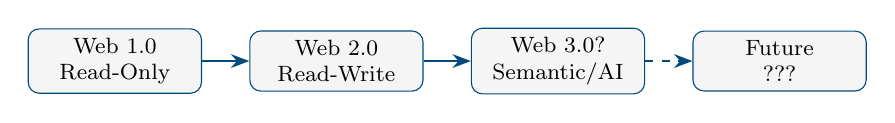
\begin{tikzpicture}[
        node distance=1cm,
        box/.style={rectangle, draw=primaryblue, fill=lightgray, rounded corners, minimum width=2.2cm, minimum height=0.7cm, align=center, font=\footnotesize}
    ]
        \node[box] (web1) {Web 1.0\\Read-Only};
        \node[box, right=0.6cm of web1] (web2) {Web 2.0\\Read-Write};
        \node[box, right=0.6cm of web2] (web3) {Web 3.0?\\Semantic/AI};
        \node[box, right=0.6cm of web3] (future) {Future\\???};
        
        \draw[-{Stealth}, thick, primaryblue] (web1) -- (web2);
        \draw[-{Stealth}, thick, primaryblue] (web2) -- (web3);
        \draw[-{Stealth}, thick, primaryblue, dashed] (web3) -- (future);
    \end{tikzpicture}
    \end{center}
\end{frame}

%------------------------------------------------------
% SLIDE 48: Conclusion: Five Revolutions, Recurring Questions
%------------------------------------------------------
\begin{frame}{Conclusion: Five Revolutions, Recurring Questions}
    \begin{itemize}
        \item Each IT revolution---writing, printing, telegraph/telephone, broadcast media, and the web---promised to democratize knowledge and connect humanity.
        \item Each also raised concerns about memory (Plato), propaganda (Luther's pamphlets, WWI), ownership (Marx), passivity (Postman), and embodiment (Dreyfus).
        \item The ethical questions recur because technology amplifies human choices: it can spread enlightenment or lies, connect or isolate, liberate or control.
        \item Understanding this history helps us ask better questions about AI, social media, and whatever comes next.
    \end{itemize}
    
    \vspace{0.3em}
    
    \begin{exampleblock}{Key Takeaway}
        Technology is never neutral. The design of information systems---who controls them, what they measure, how they shape attention---reflects and reinforces values. Studying the history of IT ethics helps us become more thoughtful creators and users of the technologies that shape our lives.
    \end{exampleblock}
    
    \vspace{0.5em}
    \centering
    \textit{``Those who cannot remember the past are condemned to repeat it.''} --- George Santayana
\end{frame}


\end{document}